% Chapter 1

\chapter*{Introduction} % Main chapter title
\addcontentsline{toc}{chapter}{Introduction}
\label{Introduction} % For referencing the chapter elsewhere, use \ref{Chapter1} 

%----------------------------------------------------------------------------------------

% Define some commands to keep the formatting separated from the content 
\newcommand{\keyword}[1]{\textbf{#1}}
\newcommand{\tabhead}[1]{\textbf{#1}}
\newcommand{\code}[1]{\texttt{#1}}
\newcommand{\file}[1]{\texttt{\bfseries#1}}
\newcommand{\option}[1]{\texttt{\itshape#1}}

%----------------------------------------------------------------------------------------

This master thesis will treat of one of the major problematic in astronomy and in optics in general, the aberrations and their corrections. We will study and develop a method to identify the static aberrations present in an  optical system using the data produced by it.

\vspace{1cm}


Ground based observation is as old as the first men. But since the Galilei Galileo telescope in 1609, the resolution power of the telescopes is far greater. Many invention lead to the construction of the largest telescopes ever built, the Very Large Telescope (VLT). Now that we are able to build enormous telescope with mirror diameter up to 8m, soon to be bitten by the Extremely Large Telescope (ELT) with its 18m, the limitation of the resolution is not the diameter anymore, but the atmosphere. Indeed, the turbulence present in the atmosphere creates a turbulent distribution of refractive index due to the distribution of temperature principally. This alters the optical path of the light through the Earth's atmosphere which finally deteriorates the images given by the telescope.

\begin{figure}
\begin{center}
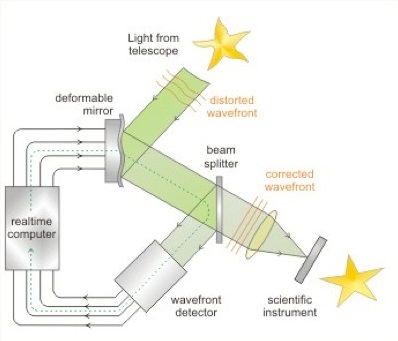
\includegraphics[width=0.4\textwidth,angle=0]{Figures/ao_scheme.jpg}
\caption{Adaptive optics schema}
source : \url{http://www.bo.astro.it/ter5/ter5/ao.html}.
\label{fig:ao_scheme}
\end{center}
\end{figure}

The first system to correct aberration in telescope where the active optics system. It consisted of actuators placed under the telescope mirrors capable of correcting the telescope deformation under the gravity effect, vibration, etc... Those systems are not fast enough to correct for the turbulence but they already improved the images. The sate-of-the-art technique is the adaptive optics, developed to counter the effects of the atmosphere. It consists of characterizing the aberrations present in the wavefront and correct them in real time. The schema of principle is shown in Figure \ref{fig:ao_scheme}. It uses a wavefront sensor to characterize the wavefront and then pass the information to a deformable mirror to correct and so on, it is called an adaptive optic loop. It works really good. But the downside of this method is that it do not correct all the aberrations up to the scientific detector, those uncorrected aberrations are called Non-Common Path Aberration (NCPA), they are generally static or slowly evolving in time. The adaptive optic also requires a complex optical system before the scientific detector. The beam is split in two. One arm goes to the scientific detector and the other is used in the adaptive optic loop.

In this work, we will present a method called phase diversity that uses images of a scientific detector to deduct the aberration present in the wavefront. In our case, we will work on the static aberrations that deform the wavefront. The phase diversity was first introduced by \citet{Gonsalves_1982}. The idea is to use one focus and one defocused image to retrieve the aberrations. Two images at least are needed due to the property of light acquisition. There is an indetermination, because the detector are only sensitive to the intensity of light and not its complex amplitude, that is raised adding a phase diversity. Unlike adaptive optic system, the phase diversity requires nearly no additional optical component depending on how it is implemented. The final aim of this project would be to integrate the developed phase diversity into the design of the DAG telescope in Turkey, see Figure \ref{fig:DAGtelescope}.

\begin{figure}
\begin{center}
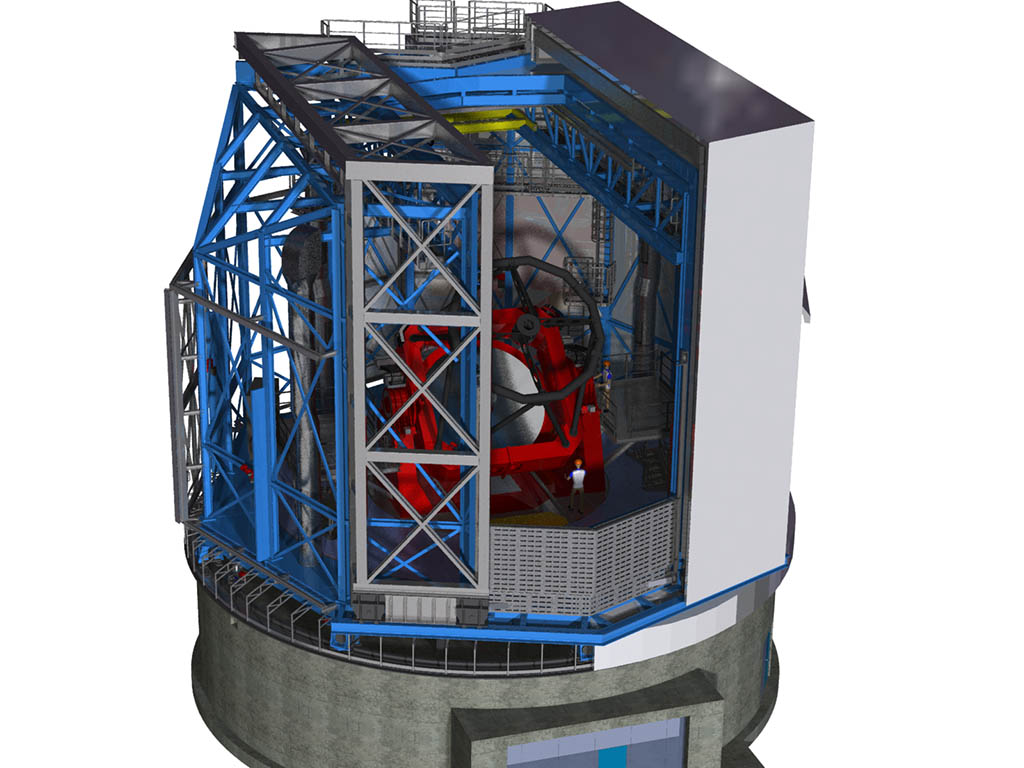
\includegraphics[width=0.5\textwidth,angle=0]{Figures/DAGtelescope.jpg} \\
\caption{DAG 4m telescope} 
source : \url{http://www.eie.it/en/progetti/dag-dogu-anadolu-gozlemevi}.
\label{fig:DAGtelescope}
\end{center}
\end{figure}

\vspace{1cm}
This report is organized as following. First, a review of the necessary theoretical background is reminded, going from the scalar theory of diffraction to the description of phase retrievals methods. Then we will present an experiment conducted in the optic laboratory at HEIG-VD. In which the ONERA algorithm of phase diversity is tested and used in comparison with a Shack-Hartmann wavefront sensor. And finally, the development of an analytical phase diversity algorithm is presented and tested with simulated PSFs.